\documentclass[12pt, a4paper]{article}

\usepackage{graphicx}
%usepackage[capitalise]{cleveref}
\usepackage{titling}


\usepackage[margin=0.8in]{geometry}
\usepackage{array}
\usepackage{cleveref}

\usepackage{fancyhdr}
\pagestyle{fancy}
\setlength{\headheight}{28pt}

\makeatletter 
\lhead{}
\chead{}
\rhead{\textbf{\@title}}
\lfoot{\@date}
\cfoot{\@author}
\rfoot{\thepage}
\renewcommand{\headrulewidth}{0.4pt}
\renewcommand{\footrulewidth}{0.4pt}
\makeatother 

\usepackage[margin=0.8in]{geometry}
\usepackage{array}
\usepackage{cleveref}
\title{Postcode Anonymity Analysis}
\author{Adam Hardy}
\date{May 2021}
\pagenumbering{gobble}% Remove page numbers (and reset to 1)

\begin{document}
\maketitle
\cleardoublepage
\pagenumbering{arabic}% Arabic page numbers (and reset to 1)

\section{Postcode Format}
\begin{table}
\begin{center}
	\begin{tabular}{ >{\centering\arraybackslash}m{0.125\textwidth} | >{\centering\arraybackslash}m{0.1\textwidth} | >{\centering\arraybackslash}m{0.1\textwidth} | >{\centering\arraybackslash}m{0.07\textwidth} | >{\centering\arraybackslash}m{0.1\textwidth} | >{\centering\arraybackslash}m{0.1\textwidth} | >{\centering\arraybackslash}m{0.1\textwidth} | >{\centering\arraybackslash}m{0.07\textwidth}}
		Postcode Format & Outward Code & Inward Code & Area & District & Sub-District & Sector & Unit \\ \hline
		AA9A9AA & AA9A & 9AA & AA & AA9 & AA9A & AA9A9 & AA \\
        A9A 9AA & A9A & 9AA & A & A9 & A9A & A9A 9 & AA \\
        A9\space\space9AA & A9 & 9AA & A & A9 & A9 & A99 & AA \\
        A99 9AA & A99 & 9AA & A & A99 & A99 & A99 & AA \\
        AA9 9AA & AA9 & 9AA & AA & AA9 & AA9 & AA9 9 & AA \\
        AA999AA & AA99 & 9AA  & AA & AA99 & AA99 & AA999 & AA\\
	\end{tabular}
\end{center}
\label{table:postcode_format}
\caption{postcode format}
\end{table}

\begin{figure}
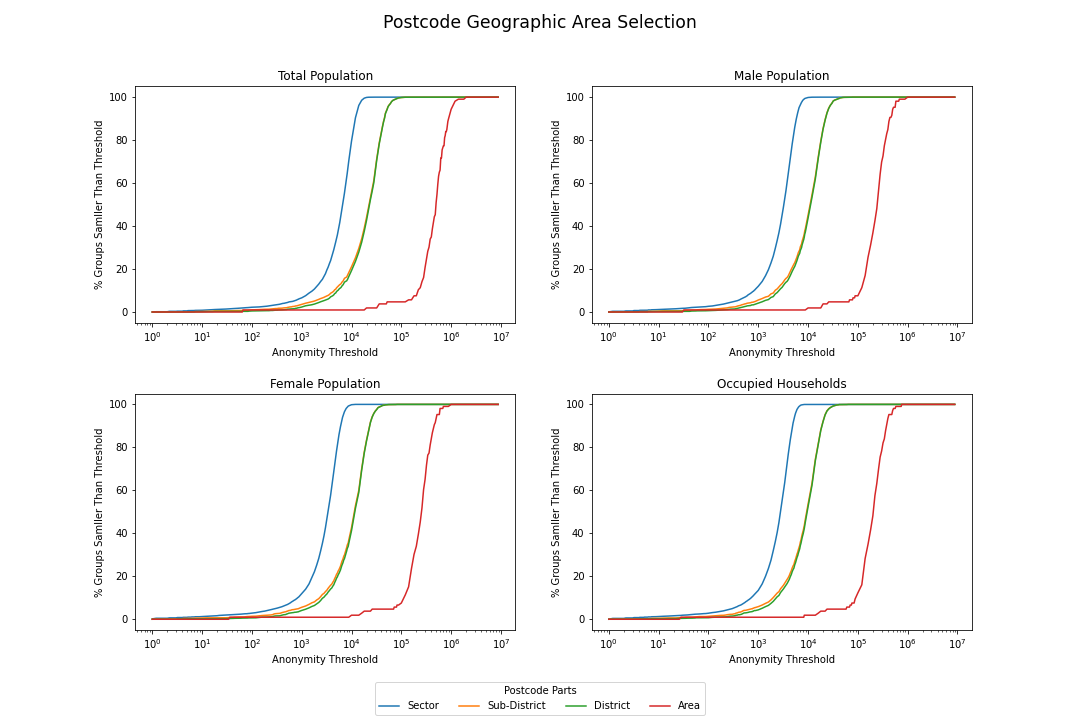
\includegraphics[width=1\textwidth,trim={0.1cm, 0.1cm, 0.1cm, 0.1cm},clip]{images/postode_selection.png}
\label{fig:postcode_selection}
\caption{postcode selection}
\end{figure}

\begin{figure}
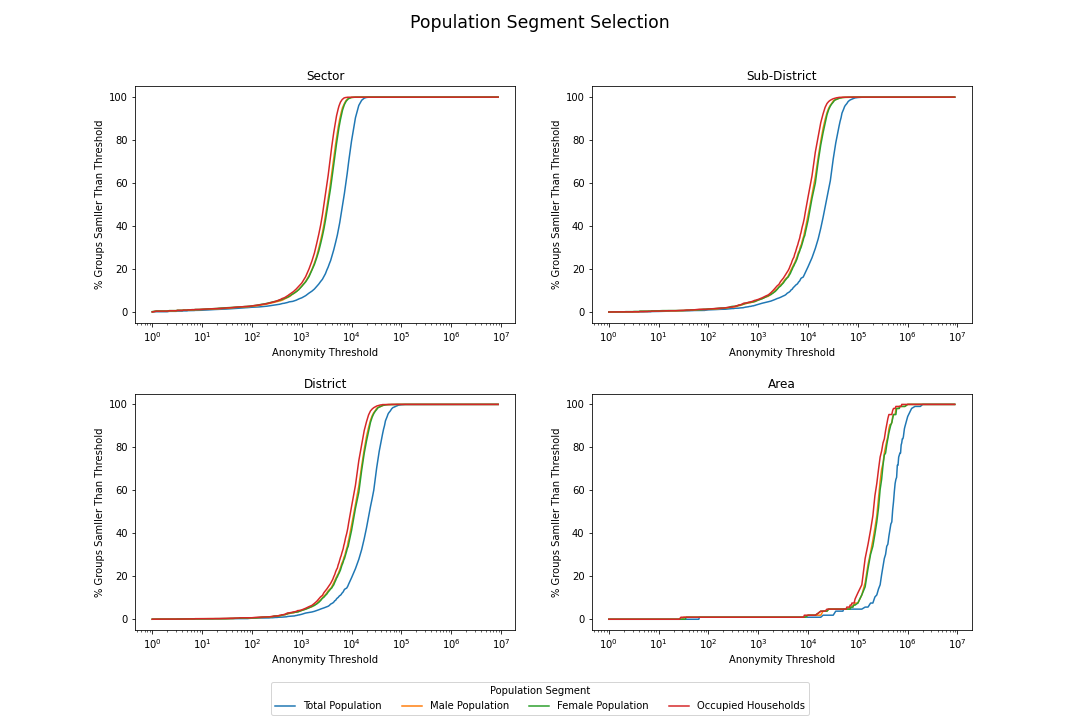
\includegraphics[width=1\textwidth,trim={0.1cm, 0.1cm, 0.1cm, 0.1cm},clip]{images/population_selection.png}
\label{fig:population_selection}
\caption{population selection}
\end{figure}

\end{document}